\documentclass[letterpaper,twocolumn,10pt]{article}
\usepackage{usenix2019_v3}

\usepackage{microtype}
\usepackage[leqno]{amsmath}
\allowdisplaybreaks
\usepackage{amssymb}
\usepackage{mathtools}
\usepackage{amsthm}
\usepackage{graphicx}
\usepackage{enumerate}
\usepackage{stmaryrd}
\usepackage{setspace}
\usepackage{stfloats}
\usepackage{tikz}
\usetikzlibrary{matrix}

\usepackage{adjustbox}
\usepackage{hyperref}
%you can add more packages using the same code above

\usepackage[color=yellow,textsize=scriptsize]{todonotes}
\usepackage{cleveref}

\setlength{\marginparwidth}{1.5cm}
%------------------

%\setlength{\topmargin}{0.0in}
%\setlength{\textheight}{10in}
%\setlength{\oddsidemargin}{0.0in}
%\setlength{\evensidemargin}{0.0in}
%\setlength{\textwidth}{6.5in}

%-------------------
\theoremstyle{definition}
\newtheorem{theorem}{Theorem}[section]
\newtheorem{proposition}[theorem]{Proposition}
\newtheorem{lemma}[theorem]{Lemma}
\newtheorem{corollary}[theorem]{Corollary}
\newtheorem{conjecture}[theorem]{Conjecture}

\newtheorem{definition}[theorem]{Definition}
\newtheorem{assumption}[theorem]{Assumption}
\newtheorem*{example}{Example}

%------------------

%Everything before begin document is called the pre-amble and sets out how the document will look
%It is recommended you don't touch the pre-amble until you are familiar with LateX

\newcommand{\AgdaId}[1]{\ensuremath{\langle #1 \rangle_\mathtt{Agda}}}
\newcommand{\defeq}{{}\triangleq{}}
\newcommand{\conj}{\mathrel\land}
\newcommand{\disj}{\mathrel\lor}

\newcommand{\awa}[2]{\hphantom{#1}\mathclap{#2}\hphantom{#1}} % as wide as

\renewcommand{\i}[1]{\ensuremath{\mathit{#1}}}
\newcommand{\id}[1]{\ensuremath{\mathit{#1}}}

\newcommand{\Spec}{\ensuremath{\mathbb S}}
\newcommand{\Prog}{\ensuremath{\mathbb P}}
\newcommand{\ProgState}{\ensuremath{\id{RawState}^{\mathbb P}}}
\newcommand{\ProgInv}{\ensuremath{\mathbb P^\dagger}}
\newcommand{\NewSpec}{\mathcal{N}_{\kern1.45pt\Spec}}
\newcommand{\NewProg}{\mathcal{N}_{\kern1.375pt\Prog}}

\newcommand{\actw}{\mathsf w}
\newcommand{\actwc}{\mathsf w^\mathsf{c}}
\newcommand{\actf}{\mathsf f}
\newcommand{\actr}{\mathsf r}
\newcommand{\actfc}{\mathsf{f^c}}
\newcommand{\actrc}{\mathsf{r^c}}
\newcommand{\actcp}{\mathsf{cp}}
\newcommand{\actes}{\mathsf{es}}
\newcommand{\actcpc}{\mathsf{cp^c}}
\newcommand{\actesc}{\mathsf{es^c}}

\newcommand{\hmid}{\hphantom{\mid{}}}

\newcommand{\ttIn}[2]{\xrightarrow{#1}_{#2}}
%%\newcommand{\ttsIn}[2]{\xrightarrow{#1}^{\raisebox{-7pt}{\scriptsize\ensuremath{*}}}_{#2}}
\newcommand{\dxrightarrow}[1]{\xrightarrow{#1}\mathrel{\mkern-14mu}\rightarrow}
\newcommand{\ttsIn}[2]{\dxrightarrow{#1}_{#2}}
\newcommand{\ttP}[1]{\ttIn{#1}{\Prog}}
\newcommand{\ttsP}[1]{\ttsIn{#1}{\Prog}}
\newcommand{\ttS}[1]{\ttIn{#1}{\Spec}}
\newcommand{\ttsS}[1]{\ttsIn{#1}{\Spec}}
\newcommand{\ttPI}[1]{\ttIn{#1}{\ProgInv}}
\newcommand{\ttsPI}[1]{\ttsIn{#1}{\ProgInv}}


\begin{document}

\title{Behavioral Correctness and Snapshot Consistency in Agda}
\author{Lin Tzu Chi \and Hsiang-Shang Ko}
%\date{}
\maketitle

\begin{abstract}
We have proved the behavioral correctness and snapshot consistency of SCFTL in Agda, assuming that some essential properties have been verified by an SMT solver.
\end{abstract}

% !TEX root = main.tex

\section{Overall Structure}

%Recall that, to simplify the proof of crash-determinacy, we introduce an abstract (and simpler) transition system~\Spec\ that acts as a specification of the actual program transition system~\Prog.
%Crash-determinacy will be established on~\Spec\ instead, and by making \Spec\ simulate~\Prog\ (a notion which we will define below), every well-formed fragment in~\Prog\ will correspond to one in~\Spec\ and be crash-deterministic.%
%\todo{define crash-determinacy on fragments, and then on transition systems}\
%The overall strategy for carrying out the proof is to use an SMT solver wherever possible, and verify the rest with a proof assistant, in this case Agda.
%More specifically, the solver establishes the preservation of invariants in~\Prog\ and the simulation of~\Prog\ by~\Spec, and then with Agda we prove that \Spec\ is crash-deterministic, and that crash-determinacy of~\Spec\ does lead to crash-determinacy of~\Prog\ due to the simulation.

In this appendix we present the content of \S4 in detail. The definitions, theorems and lemmas, and their proofs are all formalized with the Agda proof assistant, while in this appendix we omit the proofs, the details of which are all written and checked in Agda, and merely present the important definitions, theorems, and lemmas in the usual mathematical style.
Throughout this appendix we will annotate definitions, theorems, etc with the corresponding Agda identifiers enclosed in \AgdaId{\cdot}, so that readers who are proficient in Agda can look up the identifiers in the source code easily.

The Agda proof does not depend on the detail of~\Prog\ and the invariants on program states, which will be formulated as assumptions in \cref{sec:Prog}.
We will then define \Spec, formulate a generic definition of snapshot consistency and prove the snapshot consistency of \Spec\ in \cref{sec:Spec}.
Next we will formally define the simulation relation between \Prog~and~\Spec, but instead of considering the entire~\Prog, it suffices to focus on a sub-system~\ProgInv\ of~\Prog\ which consists of only the states satisfying the invariants and the transitions ``respecting'' the invariants. \ProgInv will be defined in \cref{sec:ProgInv}.
The simulation relation between \ProgInv~and~\Spec, to be defined in \cref{sec:sim}, will be easier to handle (compared to the one between \Prog~and~\Spec), and the snapshot consistency of \ProgInv\ is the same as that of \Prog\ since the property is only about multi-recovery fragments, which can be shown (in \cref{sec:ProgInv}) to be included in~\ProgInv.
Finally we will present the behavioral correctness and snapshot consistency of~\ProgInv\ in \cref{bcsc}.


% !TEX root = main.tex

\section{The Program Transition System~\Prog}
\label{sec:Prog}

We assume that three sets are given,  
$$ \AgdaId{\id{Addr}},\ \AgdaId{\id{Data}},\ \text{and}\ \AgdaId{\ProgState} $$
where $\i{Addr}$ is the set of memory addresses, $\i{Data}$ the set of values of memory cells, $\ProgState$ the set of all possible program states.
The exact definitions of these sets are irrelevant to the Agda proof and omitted.
We will need to read the memory cells in a program state, which is done by the function
$$ \AgdaId{\id{read}} : \ProgState \to (\i{Addr} \to \i{Data}) $$
which returns the mapping from memory cell addresses to their values in a program state.
We also assume that there is a predicate $\AgdaId{\id{Init}^R}$ on \ProgState\ that is used to identify the new disk states.

The (labelled) transition system~\Prog\ uses \ProgState\ as its states, and its actions (labels) are defined by
\begin{align*}
%\noalign{\center{\small{State of Prog, we don't have to know the details.}}}
	\AgdaId{\i{Action}} \defeq{} &\{\, \actw_{\i{addr}, \i{data}} \mid \i{addr} \in \i{Addr}, \i{data} \in \i{Data} \,\} \\
	\cup \ &\{\, \actwc_{\i{addr}, \i{data}} \mid \i{addr} \in \i{Addr}, \i{data} \in \i{Data} \,\}\\
	\cup \ &\{ \actf, \actr, \actcp, \actes, \actfc, \actrc, \actcpc, \actesc \}
\end{align*}
Most of the time the pair of address and data in a $\actw$ or $\actwc$ action is not important, in which case we will omit the subscript.
We will refer to a transition system whose labels are drawn from \id{Action} as a \emph{disk model} --- in particular, \Prog\ is a disk model.
The ternary (single-step) transition relation of~\Prog\ is
$$ {\ttP{}} \subseteq \ProgState \times \i{Action} \times \ProgState \qquad \AgdaId{\_\sem{\_}^{\mathrm R}{\blacktriangleright}\_} $$
Its exact definition is, again, irrelevant in this appendix and omitted.
We write
$$s \ttP{a} s'$$
when state~$s$ transits to~$s'$ through action~$a$ in~\Prog.

Recall that there are two types of invariants on the states, the representation invariant \AgdaId{\i{RI}} and the crash invariant \AgdaId{\i{CI}}, which are preserved or transformed by the transitions; these properties are proved by an SMT solver, and are made assumptions in this proof.

\begin{assumption}[per-operation correctness]
For all $s$, $s' \in \ProgState$, the following are assumed:
\begin{align*}
s \ttP{\awa{\actw}{\actw }} s' \conj \i{RI}(s) &\implies \i{RI}(s') & \AgdaId{\id{RIRI}} \\
s \ttP{\awa{\actw}{\actf }} s' \conj \i{RI}(s) &\implies \i{RI}(s')\\
s \ttP{\awa{\actw}{\actcp}} s' \conj \i{RI}(s) &\implies \i{RI}(s')\\
s \ttP{\awa{\actw}{\actes}} s' \conj \i{RI}(s) &\implies \i{RI}(s')\\
s \ttP{\awa{\actw}{\actwc}} s' \conj \i{RI}(s) &\implies \i{CI}(s') & \AgdaId{\id{RICI}} \\
s \ttP{\awa{\actw}{\actfc}} s' \conj \i{RI}(s) &\implies \i{CI}(s')\\
s \ttP{\awa{\actw}{\actcp}} s' \conj \i{RI}(s) &\implies \i{CI}(s')\\
s \ttP{\awa{\actw}{\actes}} s' \conj \i{RI}(s) &\implies \i{CI}(s')\\
s \ttP{\awa{\actw}{\actr }} s' \conj \i{CI}(s) &\implies \i{RI}(s') & \AgdaId{\id{CIRI}} \\
s \ttP{\awa{\actw}{\actrc}} s' \conj \i{CI}(s) &\implies \i{CI}(s') & \AgdaId{\id{CICI}}
\end{align*}
\end{assumption}

We also assume that the new disk states satisfy $\id{CI}$.

\begin{assumption}[\AgdaId{\ensuremath{\id{init}^R\text-\id{CI}}}]
\[ \id{Init}^R(s) \implies \id{CI}(s) \]
\end{assumption}

%Our goal, crash-determinacy on~\Prog, can be stated as follows:
%\begin{theorem}[crash-determinacy on \Prog] \label{theoremP}
%	There are two possible situations where a recovery is needed, crash at write and crash at flush, we will prove that crash-determinacy would hold in both scenarios. Thus for all $s_0, s', s'', s''' \in \i{ProgState}$, the theorem can be stated separately in two cases:
%\begin{align*}
%%Case $\actwc$: \\
%	         \intertext{Case $\actwc$:}
%	         &  s_0 \ttsP{\i{((\actw \lor \actf)\ast)} \actf} s' \conj s' \ttsP{\i{(\actw \ast)} \actwc \i{(\actrc\ast)} \actr} s'' \\
%	\implies & \i{read(s')} \equiv \i{read(s'')} \\
%	         \intertext{Case $\actfc$:}
%	         & s_0 \ttsP{\i{((\actw \lor \actf)\ast)} \actf} s' \conj s' \ttsP{\i{(\actw \ast)}} s'' \conj s'' \ttsP{\actfc \i{(\actrc \ast)} \actr} s'''  \\
%	\implies & \i{read(s')} \equiv \i{read(s''')} \disj \i{read(s'')} \equiv \i{read(s''')} 
%\end{align*}
%\end{theorem}
%where $s_0$ is an initial state in \Prog.
%To prove the theorem, we would need to introduce two other transition systems~\Spec~and~\ProgInv.


% !TEX root = main.tex

\section{The Specification Transition System~\Spec}
\label{sec:Spec}

For the disk model~\Spec, its states are those in the set
$$ \AgdaId{\SpecState} \defeq (\i{Addr} \to \i{Data}) \times (\i{Addr} \to \i{Data}) \times \mathbb N $$
each of which contains a pair of mappings from \i{Addr} to \i{Data} and a natural number; these two mappings represent the volatile and stable parts of a state in the specification, and the natural number is the write count.
Similarly to $\i{read}$ in \Prog, the functions
\begin{align*}
\i{volatile} &: \SpecState \to (\i{Addr} \to \i{Data}) & \AgdaId{\id{State}.\id{volatile}} \\
\i{stable} &: \SpecState \to (\i{Addr} \to \i{Data}) & \AgdaId{\id{State}.\id{stable}}
\end{align*}
extract the respective mappings from a \Spec-state.
The new states of~\Spec\ are characterized by the predicate $\AgdaId{\id{Init}(s)} \defeq \forall a.\ \id{stable}(s)(a) = \id{defaultData}$ where $\AgdaId{\id{defaultData}} \in \id{Data}$ is some default value for memory cells.
The transition relation
$$ {\ttS{}} \subseteq \SpecState \times \i{Action} \times \SpecState \qquad \AgdaId{\_\sem{\_}{\blacktriangleright}\_} $$
has been defined in figure~4 in the main text.

Next we state snapshot consistency generically for disk models.
To do so we will need to talk about sequences of transitions and particular forms of traces (i.e., sequences of actions, which are of type $\AgdaId{\id{Trace}}$), and some general definitions will be helpful.
Then we are able to prove the snapshot consistency on \Spec.

\begin{definition}[fragments, \AgdaId{\id{RTC}}]\label{def:frag}
Let $T = (S, \Lambda, \ttIn{}{})$~be a labelled transition system.
A \emph{fragment} in~$T$ is a sequence of transitions
$$ s_0 \ttIn{a_1}{} s_1 \ttIn{a_2}{} \cdots \ttIn{a_n}{} s_n $$
where $s_i \in S$ and $a_j \in \Lambda$ for all $i$~and~$j$.
We sometimes omit the intermediate states and write
$$ s_0 \ttsIn{a_1,\,a_2,\,\ldots,\,a_n}{} s_n $$
Note that a fragment may contain no transitions, in which case the starting and ending states are the same: 
$$ s_0 \ttsIn{\vphantom{a_n}}{} s_0 $$
\end{definition}

\begin{definition}[one-recovery traces, \AgdaId{\id{OneRecovery}}]
A \emph{one-recovery} trace has one of the following forms:
\begin{itemize}
\item $a_1, \ldots, a_{k-1}, \actf, b_1, \ldots, b_\ell, \actwc, (\actrc)^m, \actr$\quad,
\item $a_1, \ldots, a_{k-1}, \actf, b_1, \ldots, b_\ell, \actfc, (\actrc)^m, \actr$\quad,
\item $b_1, \ldots, b_\ell, \actwc, (\actrc)^m, \actr$\quad, and
\item $b_1, \ldots, b_\ell, \actfc, (\actrc)^m, \actr$\quad,
\end{itemize}
where $a_i$~are successful regular or snapshot operations and $b_j$~are successful regular operations.
\end{definition}
This is the trace part of one-recovery fragments defined in the main text, expanded to four cases to simplify the subsequent proof structure.

\begin{definition}[multi-recovery traces, \AgdaId{\id{MultiRecovery}}]
The set of \emph{multi-recovery} traces is inductively defined by the following two rules:
\begin{itemize}
\item a trace of the form $(\actrc)^m\,\actr$ is a multi-recovery trace, and
\item the concatenation $\id{tr}, \id{tr}'$ of a multi-recovery trace $\id{tr}$ and a one-recovery trace $\id{tr}'$ is a multi-recovery trace.
\end{itemize}
\end{definition}

Note that, differently from the main text, the two notions above are defined on traces rather than fragments; to reconcile the difference, we will say that a fragment is one-/multi-recovery when its trace is one-/multi-recovery.
Also note that the definition of multi-recovery fragments in this appendix is more specific than that in the main text (where the first state is required to be new and there are some trailing transitions), but below we will state our theorems in a way that makes them apply to the multi-recovery fragments as defined in the main text.

\begin{definition}[snapshot consistency of a one-recovery fragment, \AgdaId{\id{SnapshotConsistency}}]
A one-recovery fragment~$\id{fr}$ is \emph{snapshot-consistent} under an equivalence relation~$\id{ER}$ if
\begin{itemize}
\item $\id{ER}(s_2, s_4)$ \\
when $\id{fr} = s_1 \ttsIn{a_1,\, \ldots,\, a_{k-1}}{} s_2 \ttsIn{\actf,\, b_1,\, \ldots,\, b_\ell,\, \actwc,\, (\actrc)^m,\, \actr}{} s_4$,
\item $\id{ER}(s_3, s_4)$ or $\id{ER}(s_2, s_4)$ \\
when $\id{fr} = s_1 \ttsIn{a_1,\, \ldots,\, a_{k-1}}{} s_2 \ttsIn{\actf,\, b_1,\, \ldots,\, b_\ell}{} s_3 \ttsIn{\actfc,\, (\actrc)^m,\, \actr}{} s_4$,
\item $\id{ER}(s_2, s_4)$ \\
when $\id{fr} = s_2 \ttsIn{b_1,\, \ldots,\, b_\ell,\, \actwc,\, (\actrc)^m,\, \actr}{} s_4$, or
\item $\id{ER}(s_3, s_4)$ or $\id{ER}(s_2, s_4)$ \\
when $\id{fr} = s_2 \ttsIn{b_1,\, \ldots,\, b_\ell}{} s_3 \ttsIn{\actfc,\, (\actrc)^m,\, \actr}{} s_4$.
\end{itemize}
\end{definition}

\begin{theorem}[snapshot consistency of \Spec, \AgdaId{\id{Spec}.\id{SC}}]\label{cdS}
For every fragment $t_0 \ttsIn{\id{tr}}{} t_1 \ttsIn{\id{tr}'}{} t_2$ in~\Spec\ where $\id{Init}(t_0)$ holds, $\id{tr}$ is multi-recovery, and $\id{tr}'$~is one-recovery, the sub-fragment $t_1 \ttsIn{\id{tr'}}{} t_2$ is snapshot-consistent under the equivalence relation $\id{ER}(t, t') \defeq \id{volatile}(t) = \id{volatile}(t')$.
\end{theorem}
%\begin{proof}[Proof of case\ \i{\actwc}.]
%	$s'$ is transited from some $s \in \i{SpecState}$ by \i{\ttS{\actf}}, so
%		$$\i{volatile(s')} \equiv \i{volatile(s)} \equiv \i{stable(s')}$$
%	since any state transited by \i{\ttS{\actw}} , \i{\ttS{\actwc}} or \i{\ttS{\actrc}} has its stable unchanged from the state it's transited from, there is an intermediate state $s'_i$ such that
%		$$s' \ttsS{\i{(\actw\ast)} \actwc \i{(\actrc*)}} s'_i \conj s'_i \ttS{\actr} s'' \conj stable(s') \equiv stable(s'_i)$$
%	, by \i{\ttS{\actr}} we know that $\i{stable(s'_i) \equiv volatile(s'')}$, thus we have
%		$$\i{volatile(s') \equiv stable(s') \equiv stable(s'_i) \equiv volatile(s'')}$$
%\end{proof}
%\begin{proof}[Proof of case\ \i{\actfc}]
%	We can find two intermediate state $s''_i$, $s''_j$ , such that $$s'' \ttS{\actfc} s''_i \conj s''_i \ttsS{\actrc*} s''_j \conj s''_j  \ttS{\actr} s'''$$
%	then by case analysis on $s'' \ttS{\actfc} s''_i$, we know that either $$\i{volatile(s'') \equiv stable(s''_i)}$$ or $$\i{stable(s'') \equiv stable(s''_i)}$$
%	if $\i{volatile(s'') \equiv stable(s''_i)}$, by substituting $s'$ with $s''$ in
%	\mbox{case-$\actwc$}, we can obtain $$\i{volatile(s'') \equiv volatile(s''')}$$
%	if $\i{stable(s'') \equiv stable(s''_i)}$, the proof is exactly the same with \mbox{case-$\actwc$}, thus $$\i{volatile(s') \equiv volatile(s''')}$$
%\end{proof}

On the surface this theorem may appear weaker than the one claimed in the main text, but we can easily show that every one-recovery sub-fragment $\id{fr}$ in a multi-recovery fragment is snapshot-consistent by applying the theorem to the sub-fragment ending with $\id{fr}$, so this theorem is in fact general enough.
The theorem, combined with the simulation between \Spec~and~\ProgInv, will be used to establish the proof of the snapshot consistency of~\ProgInv\ in later sections.

% !TEX root = main.tex

\section{The Sub-System~\ProgInv\ with Invariants}
\label{sec:ProgInv}
\ProgInv\ is a disk model whose set of states~\AgdaId{\ProgInvState}\ is a subset of \ProgState\ --- states that satisfy either $\id{RI}$~or~$\id{CI}$.
%We define \ProgInv\ because, as we will see, all the multi-recovery fragments in~\Prog\ are included in \ProgInv.
%In other words, the states in these fragments always satisfy either \i{RI} or \i{CI}.
%Thus it suffices to define a simulation of \ProgInv\ by \Spec\ to prove the behavioral correctness on~\ProgInv, from which the snapshot consistency of~\Prog\ could be derived.

The states of \ProgInv\ is defined as follows:
$$\ProgInvState \defeq{} \{\, s \in \ProgState \mid \i{RI(s) \lor CI(s)} \,\}$$
The transition relation of~\ProgInv,
$$\ttPI{} \subseteq \i{State^P} \times \i{Action} \times \i{State^P} \qquad \AgdaId{\_\sem{\_}^P{\blacktriangleright}\_} $$
which is, similarly, a subset of \i{\ttP{}}, is defined by
\begin{alignat*}{3}
	\ttPI{\awa{w}{\actw_{a, d}}} \defeq{}& \{\, (s, s') \mid s \ttP{\awa{w}{\actw_{a, d}}} s' \conj \i{RI(s)} \conj \i{RI(s')} \,\} \\
	\ttPI{\awa{w}\actf} \defeq{}& \{\, (s, s') \mid s \ttP{\awa{w}\actf} s' \conj \i{RI(s)} \conj \i{RI(s')} \,\} \\
    \ttPI{\awa{w}\actcp} \defeq{}& \{\, (s, s') \mid s \ttP{\awa{w}\actcp} s' \conj \i{RI(s)} \conj \i{RI(s')} \,\} \\
    \ttPI{\awa{w}\actes} \defeq{}& \{\, (s, s') \mid s \ttP{\awa{w}\actes} s' \conj \i{RI(s)} \conj \i{RI(s')} \,\} \\
	\ttPI{\awa{w}\actr} \defeq{}& \{\, (s, s') \mid s \ttP{\awa{w}\actr} s' \conj \i{CI(s)} \conj \i{RI(s')} \,\} \\
	\ttPI{\awa{w}{\actwc_{a, d}}} \defeq{}& \{\, (s, s') \mid s \ttP{\awa{w}{\actwc_{a, d}}} s' \conj \i{RI(s)} \conj \i{CI(s')} \,\} \\
	\ttPI{\awa{w}\actfc} \defeq{}& \{\, (s, s') \mid s \ttP{\awa{w}\actfc} s' \conj \i{RI(s)} \conj \i{CI(s')} \,\} \\
	\ttPI{\awa{w}\actcpc} \defeq{}& \{\, (s, s') \mid s \ttP{\awa{w}\actcpc} s' \conj \i{RI(s)} \conj \i{CI(s')} \,\} \\
	\ttPI{\awa{w}\actesc} \defeq{}& \{\, (s, s') \mid s \ttP{\awa{w}\actesc} s' \conj \i{RI(s)} \conj \i{CI(s')} \,\} \\
	\ttPI{\awa{w}\actrc} \defeq{}& \{\, (s, s') \mid s \ttP{\awa{w}\actrc} s' \conj \i{CI(s)} \conj \i{CI(s')} \,\} 
\end{alignat*}

From \cref{peropb}, we can prove that every multi-recovery fragment which starts from a new disk state in~\Prog\ is also one in~\ProgInv, where a new disk state in \ProgInv\ is characterized by the predicate $\AgdaId{\ensuremath{\id{Init^P(s)}}} \defeq \id{Init^R(s)} \land \id{CI(s)}$, so when considering only such fragments in~\Prog, which are ranged over by the statements of behavioral correctness and snapshot consistency, we can work with~\ProgInv\ instead.
\begin{lemma}[\AgdaId{\id{lift\text-mr}}]
For every multi-recovery fragment $s \ttsP{\id{tr}} s'$ where $\id{Init^R(s)}$ holds, there exists a fragment $s \ttsPI{\id{tr}} s'$ such that $\id{Init^P(s)}$, $\id{CI(s)}$, and $\id{RI(s')}$ hold.
\end{lemma}

%Snapshot consistency of \ProgInv, which is exactly the same with snapshot consistency of \Prog\ except the states and transition relation it applies to, can be stated as follows.
%\begin{lemma}[crash-determinacy on \ProgInv] \label{theoremPI}
%	For all~$s_0, s', s'', s''' \in \i{ProgState^\dagger}$, following two cases hold:
%\begin{align*}
%	\intertext{Case $\actwc$:}
%	&s_0 \ttsPI{\i{((\actw \lor \actf)\ast)} \actf} s' \conj s' \ttsPI{\i{(\actw\ast)} \actwc \i{(\actrc\ast)} \actr} s'' \\
%	\implies & \i{read(s')} \equiv \i{read(s'')} \\
%	\intertext{Case $\actfc$:}
%	& s_0 \ttsPI{\i{((\actw \lor \actf)\ast)} \actf} s' \conj s' \ttsPI{\i(\actw \ast)} s'' \conj s'' \ttsPI{\actfc \i{(\actrc \ast)} \actr} s''' \\
%	\implies &\i{read(s')} \equiv \i{read(s''')} \disj \i{read(s'')} \equiv \i{read(s''')}
%\end{align*}
%\end{lemma}
%Note that even this lemma is not provable yet, we will prove it later along with \cref{theoremP} once we have the simulation relations defined in next section.


% !TEX root = main.tex

\section{Simulation of~\ProgInv\ by~\Spec}
\label{sec:sim}
To establish \cref{theoremP}, we first have to define simulation between \Spec\ and \Prog, from which the behavioral correctness  can be proved, which derives the snapshot consistency on \Prog. Two kinds of abstraction relations, normal abstraction relation $\AgdaId{\i{AR}}$ and crashed abstraction relation $\AgdaId{\i{CR}}$, which are transformed or preserved on states that satisfies certain invariants(i.e. states in \ProgInv), have been proved with an SMT solver, thus are made assumptions.
\begin{assumption}[per operation correctness]\label{PerOpCorrect}
	For all $s, s' \in \ProgInvState$, $t, t' \in \SpecState$, the following are assumed:
\begin{align*}
s \ttPI{\awa{\actw}{\actw }} s' \conj t \ttS{\awa{\actw}{\actw }} t' \conj \i{AR}(s, t) &\implies \i{AR}(s', t') \tag*{\AgdaId{\id{ARAR}}}\\
s \ttPI{\awa{\actw}{\actf }} s' \conj t \ttS{\awa{\actw}{\actf }} t' \conj \i{AR}(s, t) &\implies \i{AR}(s', t')\\
s \ttPI{\awa{\actw}{\actcp}} s' \conj t \ttS{\awa{\actw}{\actcp}} t' \conj \i{AR}(s, t) &\implies \i{AR}(s', t')\\
s \ttPI{\awa{\actw}{\actes}} s' \conj t \ttS{\awa{\actw}{\actes}} t' \conj \i{AR}(s, t) &\implies \i{AR}(s', t')\\
s \ttPI{\awa{\actw}{\actwc}} s' \conj t \ttS{\awa{\actw}{\actwc}} t' \conj \i{AR}(s, t) &\implies \i{CR}(s', t')\tag*{\AgdaId{\id{ARCR}}}\\
s \ttPI{\awa{\actw}{\actfc}} s' \conj t \ttS{\awa{\actw}{\actfc}} t' \conj \i{AR}(s, t) &\implies \i{CR}(s', t')\\
s \ttPI{\awa{\actw}{\actcpc}} s' \conj t \ttS{\awa{\actw}{\actcpc}} t' \conj \i{AR}(s, t) &\implies \i{CR}(s', t')\\
s \ttPI{\awa{\actw}{\actesc}} s' \conj t \ttS{\awa{\actw}{\actesc}} t' \conj \i{AR}(s, t) &\implies \i{CR}(s', t')\\
s \ttPI{\awa{\actw}{\actr }} s' \conj t \ttS{\awa{\actw}{\actr }} t' \conj \i{CR}(s, t) &\implies \i{AR}(s', t')\tag*{\AgdaId{\id{CRAR}}}\\
s \ttPI{\awa{\actw}{\actrc}} s' \conj t \ttS{\awa{\actw}{\actrc}} t' \conj \i{CR}(s, t) &\implies \i{CR}(s', t')\tag*{\AgdaId{\id{CRCR}}}
\end{align*}
\end{assumption}
For proof convenience, we define simulation relation between a state in \ProgInvState\ and a state in \SpecState\ as either $\i{AR}$ or $\i{CR}$ holds between them.
\begin{definition}[simulation relation, \AgdaId{\id{SR}}]
    $$\i{SR(s, t)} \defeq \i{AR(s, t)} \lor \i{CR(s, t)}$$
\end{definition}
As well proved with an SMT solver, for every pair of \i{s \in \ProgInvState} and \i{t \in \SpecState} that satisfies the normal abstraction relation $AR(s,t)$, \emph{observational equivalence} holds, that the content of~$s$ is equivalent to the content of the volatile part of~$t$.
\begin{assumption}[\AgdaId{\id{AR{\Rightarrow}ObsEquiv}}]\label{ObsEquiv}
	$$
	 \forall \i{s} \in \ProgInvState,t \in \SpecState \ldotp
	 \i{AR(s, t)} \implies \i{read(s)} \equiv \i{volatile(t)}
	$$
\end{assumption}

Then we can state that the simulation relation is preserved between \Prog\ and~\Spec. 

\begin{lemma}[\AgdaId{\id{runSimSR}}]\label{lemma-1}
%    If $\i{SR}$ holds between a pair of states $s \in \ProgInvState$ and $t \in \SpecState$, and~$s'~\in~\ProgInvState$ is a state after a sequence of actions performed on~$s$, there always exists a state  $t' \in \SpecState$ such that $\i{SR}$ between~$t$~and~$t'$ holds, while $t'$ is a state after the same sequence of actions performed on $t$.
	\begin{align*}
		&\forall s, s' \in \ProgInvState, t \in \SpecState, \i{tr} \in \i{Trace} \ldotp\\
		&\qquad \qquad s \ttsPI{\i{tr}} s'  \conj \i{SR(s, t)} \implies \exists t' \ldotp t \ttsS{\i{tr}} t' \conj \i{SR(s', t')} \\
	\end{align*}
\end{lemma}
%	\begin{onehalfspacing}
%\begin{proof}
%	\todo{elaborate why there is always a next state.}
%	There exists $t' \in SpecState$, such that $t \ttsS{\i{ef}} t'$, and by applying \cref{PerOpCorrect} repeatedly, we know that~$\i{s \ttsPI{\i{ef}} s'}$, $\i{t \ttsS{\i{ef}} t'}$ and~$\i{AR(s, t)} \lor \i{CR(s, t)}$ implies either~$\i{AR(s', t')}$ or~$\i{CR(s', t')}$, as sketched in \cref{fig:sketch1}.
%\end{proof}
%	\end{onehalfspacing}
	\begin{figure}[h] \centering
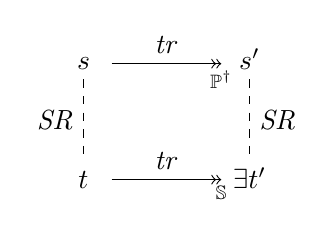
\begin{tikzpicture}
  \matrix (m) [matrix of math nodes,row sep=3em,column sep=4em,minimum width=2em]
  {
	  s & \vphantom{s}\smash{s'} \\
	 t & \vphantom{t}\smash{\exists t'} \\};
  \path[-stealth]
	(m-1-1) edge [dashed, -] node [left] {$\i{SR}$} (m-2-1)
			edge [->>] node [midway, above] {$ \i{tr} $} node [at end, below=-0.1em] {\scriptsize{\ProgInv}}  (m-1-2)
	(m-2-1) edge [->>] node [midway, above] {$ \i{tr} $} node [at end, below=-0.1em] {\scriptsize{\Spec}} (m-2-2)
	(m-1-2) edge [dashed, -] node [right] {$\i{SR}$} (m-2-2);
\end{tikzpicture}
		\caption{Illustration diagram of \cref{lemma-1}}
\label{fig:sketch1}
	\end{figure}

Note that, our goal is to establish behavioral correctness and snapshot consistency of multi-recovery fragments defined in the main text, whose traces are of the form $$(r^c)^m, r, \i{tr}_1,...,\i{tr}_n,\i{tr'}$$, where $\i{tr}_1,...,\i{tr}_n$ are one-recovery fragments, and $\i{tr'}$ is a trailing fragment without any crashes.
To better illustrate behavioral correctness, we define two multi-recovery fragments with the same trace, one in \Prog\ and one in~\Spec, to be $\AgdaId{\i{Conformant}}$ if for every pair of corresponding states, in the sense that they are both the states after the same action at a specific position in that trace is performed, are observationally equivalent.\\
Since a multi-recovery fragment consists of multiple one-recovery fragments, we define $\AgdaId{\i{Conformant{\text-}1R}}$ to describe conformance particularly between two one-recovery fragments, and $\AgdaId{\i{Conformant{\text-}all}}$ to describe conformance between two fragments where every action in the trace is successful(i.e. without crashes).\\
\begin{definition}[\i{Conformance{\text-}1R}]
    For two fragments $\i{frP} = s \ttsPI{\i{tr, a}} s'$ and $\i{frS} = t \ttsS{\i{tr, a}} t'$, $\i{Conformance{\text-}1R}(\i{frP}, \i{frS})$ holds if both of the following hold:
    \begin{itemize}
        \item $\i{frP'} = s \ttsPI{\i{tr}} s''$ and $\i{frS'} = t \ttsS{\i{tr}} t''$ satisfy \i{Conformance{\text-}1R(frP', frS')}
    \end{itemize}
\end{definition}

\begin{definition}[\i{Conformance{\text-}all}]
    For two fragments $\i{frP} = s \ttsPI{\i{tr, a}} s'$ and $\i{frS} = t \ttsS{\i{tr, a}} t'$ where $\i{tr, a}$ are all successful actions, \i{Conformance{\text-}all} holds for \i{frP} and \i{frS} if both of the following hold:
    \begin{itemize}
        \item $\i{frP'} = s \ttsPI{\i{tr}} s''$ and $\i{frS'} = t \ttsS{\i{tr}} t''$ satisfy Conformance{\text-}all(frP', frS')

    \end{itemize}
\end{definition}

\begin{theorem}[behavioral correctness, $\AgdaId{\i{BC}}$]   
For all fragments $\i{frP_1} = s \ttsPI{\i{tr}} s'$ and $\i{frP_2} = s' \ttsPI{\i{tr'}} s''$ where $\i{tr}$ is a multi-recovery trace and $\i{tr'}$ is a trace without crashes, there exist two corresponding fragments $\i{frS_1} = t \ttsS{\i{tr}} t'$ and $\i{frS_2} = t' \ttsS{\i{tr'}} t''$ such that $\i{frP_1}$ and $\i{frS_1}$ satisfy $\i{Conformant}$, while $\i{frP_2}$ and $\i{frS_2}$ satisfy $\i{Conformant{\text-}all}$. 
\end{theorem}

\section{Proof of Crash-Determinacy}
\label{sec:proof}
\begin{proof}[Proof of case \i{\actwc} in\ \cref{theoremPI}]
	We can safely assume that there exists $\i{t_0} \in \i{SpecState}$ such that $\i{AR(s_0, t_0)}$, then by repeatedly applying \cref{lemma-1} to the first relation, we have $\i{AR(s, t)}$ and $\i{AR(s', t')}$, as sketched in \cref{fig:casewPI1}.
	\begin{figure} [b] \centering
			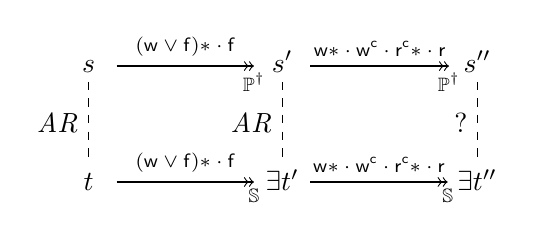
\begin{tikzpicture}
			\matrix (m) [matrix of math nodes, row sep=3em, column sep=5em, minimum width=2em]
			{ s & \vphantom{s}\smash{s'} & \vphantom{s}\smash{s''} \\
			  t & \vphantom{t}\smash{\exists t'} & \vphantom{t}\smash{\exists t''} \\};
			\path[-stealth]
			(m-1-1) edge [dashed, -] node [left] {$\i{AR}$} (m-2-1)
					edge [->>] node [above] {\scriptsize{$ \i{(\actw \lor \actf)*} \cdot \actf $}}
							   node [at end, below=-0.1em] {\scriptsize{\ProgInv}} (m-1-2)
			(m-2-1) edge [->>] node [above] {\scriptsize{$\i{(\actw \lor \actf)*} \cdot \actf$}}
							   node [at end, below=-0.1em] {\scriptsize{\Spec}} (m-2-2)
			(m-1-2) edge [dashed, -] node [left] {$\i{AR}$} (m-2-2)
					edge [->>] node [above] {\scriptsize{$\i{\actw*} \cdot \actwc \cdot \i{\actrc*} \cdot \actr$}}
							   node [at end, below=-0.1em] {\scriptsize{\ProgInv}} (m-1-3)
			(m-2-2) edge [->>] node [above] {\scriptsize{$\i{\actw*} \cdot \actwc \cdot \i{\actrc*} \cdot \actr$}}
							   node [at end, below=-0.1em] {\scriptsize{\Spec}} (m-2-3)
			(m-1-3) edge [dashed, -] node [left] {?} (m-2-3);

		\end{tikzpicture}

		\caption{Incomplete proof sketch of case \i{\actwc} of \cref{theoremPI}}
		\label{fig:casewPI1}
	\end{figure}\\
	We can find some intermediate states $s'_1$, $s'_2$, $s'_3$ by \cref{def:frag}, and by applying \cref{lemma-1} repeatedly to obtain \cref{casewPI2}.
	\begin{figure*}[h] \centering
			    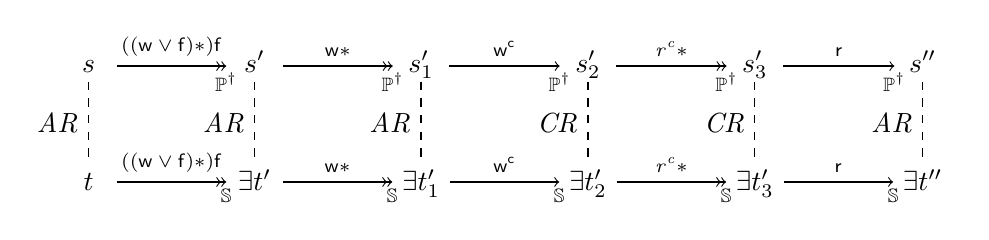
\begin{tikzpicture}
			\matrix (m) [matrix of math nodes, row sep=3em, column sep=4em, minimum width=2em]
			{ s & \vphantom{s}\smash{s'} & \vphantom{s}\smash{s'_1} & \vphantom{s}\smash{s'_2} & \vphantom{s}\smash{s'_3} & \vphantom{s}\smash{s''} \\
			  t & \vphantom{t}\smash{\exists t'} & \vphantom{t}\smash{\exists t'_1} & \vphantom{t}\smash{\exists t'_2} & \vphantom{t}\smash{\exists t'_3} & \vphantom{t}\smash{\exists t''} \\ };
			\path[-stealth]
			(m-1-1) edge [dashed, -] node [left] {$\i{AR}$} (m-2-1)
					edge [->>] node [above] {\scriptsize{$\i{((\actw \lor \actf)*)} \actf $}} node [at end, below=-0.1em] {\scriptsize{\ProgInv}} (m-1-2)
			(m-2-1) edge [->>] node [above] {\scriptsize{$\i{((\actw \lor \actf)*)} \actf $}} node [at end, below=-0.1em] {\scriptsize{\Spec}} (m-2-2)
			(m-1-2) edge [dashed, -] node [left] {$\i{AR}$} (m-2-2)
					edge [->>] node [above] {\scriptsize{$\i{\actw*}$}} node [at end, below=-0.1em] {\scriptsize{\ProgInv}} (m-1-3)
			(m-2-2) edge [->>] node [above] {\scriptsize{$\i{\actw*}$}} node [at end, below=-0.1em] {\scriptsize{\Spec}} (m-2-3)
			(m-1-3) edge [dashed, -] node [left] {$\i{AR}$} (m-2-3)
					edge [->] node [above] {\scriptsize{$\i{\actwc}$}} node [at end, below=-0.1em] {\scriptsize{\ProgInv}} (m-1-4)
			(m-2-3) edge [->] node [above] {\scriptsize{$\i{\actwc}$}} node [at end, below=-0.1em] {\scriptsize{\Spec}} (m-2-4)
			(m-1-4) edge [dashed, -] node [left] {$\i{CR}$} (m-2-4)
					edge [->>] node [above] {\scriptsize{$\i{r^c*}$}} node [at end, below=-0.1em] {\scriptsize{\ProgInv}} (m-1-5)
			(m-2-4) edge [->>] node [above] {\scriptsize{$\i{r^c*}$}} node [at end, below=-0.1em] {\scriptsize{\Spec}} (m-2-5)
			(m-1-5) edge [dashed, -] node [left] {$\i{CR}$} (m-2-5)
					edge [->] node [above] {\scriptsize{$ \i{\actr}$}} node [at end, below=-0.1em] {\scriptsize{\ProgInv}} (m-1-6)
			(m-2-5) edge [->] node [above] {\scriptsize{$ \i{\actr}$}} node [at end, below=-0.1em] {\scriptsize{\Spec}} (m-2-6)
			(m-1-6) edge [dashed, -] node [left] {$\i{AR}$} (m-2-6);

		\end{tikzpicture}

		\caption{Complete proof sketch of case \i{\actwc} of \cref{theoremPI}}
		\label{casewPI2}
	\end{figure*}
	The proof then can be completed by mapping the states in \i{ProgState^\dagger} to states in \i{SpecState} by observational equivalence (\cref{ObsEquiv}), thus crash-determinancy on \Spec\ (\cref{cdS}) entails crash-determinancy on \ProgInv:
\begin{align*}
	\i{read(s')}   &\equiv \i{volatile(t')}   \tag{by \cref{ObsEquiv}} \\
	& \qquad \quad \rotatebox{90}{$\equiv$} \tag{by \cref{cdS}}\\
	\i{read(s'')} &\equiv \i{volatile(t'')} \tag{by \cref{ObsEquiv}}
\end{align*}
\end{proof} 
\begin{proof}[Proof of case $\actfc$ in \cref{theoremPI}]
	Similarly to proof of case $\actwc$, we can find $t_0 \in \i{SpecState}$ such that $\i{AR(s_0, t_0)}$, and some states $s''_1, s''_2$ by \cref{def:frag} to obtain \cref{casefPI2}.
	By \cref{cdS}, either $\i{volatile(s')} \equiv \i{volatile(s''')}$ or $\i{volatile(s'')} \equiv \i{volatile(s''')}$. If $\i{volatile(s')} \equiv \i{volatile(s''')}$,
	\begin{align*}
	\i{read(s')}   &\equiv \i{volatile(t')} \tag{by \cref{ObsEquiv}} \\
	& \qquad \quad \rotatebox{90}{$\equiv$} \tag{by \cref{cdS}}\\
	\i{read(s''')} &\equiv \i{volatile(t''')} \tag{by \cref{ObsEquiv}}
	\end{align*}
	Similarly, if $\i{volatile(s'')} \equiv \i{volatile(s''')}$,
	\begin{align*}
	\i{read(s'')}   &\equiv \i{volatile(t'')} \tag{by \cref{ObsEquiv}} \\
	& \qquad \quad \rotatebox{90}{$\equiv$} \tag{by \cref{cdS}}\\
	\i{read(s''')} &\equiv \i{volatile(t''')} \tag{by \cref{ObsEquiv}}
	\end{align*}
	\begin{figure*}[h] \centering
		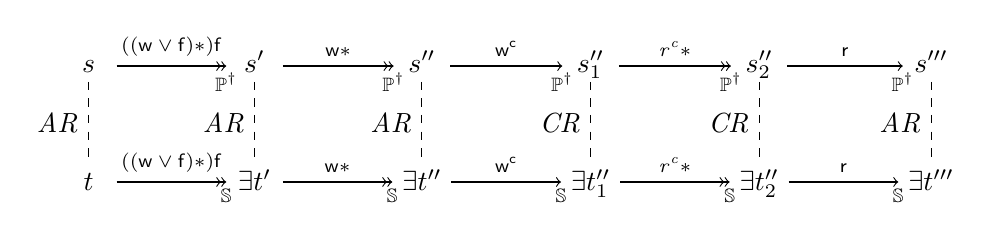
\begin{tikzpicture}
		\matrix (m) [matrix of math nodes, row sep=3em, column sep=4em, minimum width=2em]
		{ s & \vphantom{s}\smash{s'} & \vphantom{s}\smash{s''} & \vphantom{s}\smash{s''_1} & \vphantom{s}\smash{s''_2} & \vphantom{s}\smash{s'''} \\
			t & \vphantom{t}\smash{\exists t'} & \vphantom{t}\smash{\exists t''} & \vphantom{t}\smash{\exists t''_1} & \vphantom{t}\smash{\exists t''_2} & \vphantom{t}\smash{\exists t'''} \\ };
		\path[-stealth]
		(m-1-1) edge [dashed, -] node [left] {$\i{AR}$} (m-2-1)
		edge [->>] node [above] {\scriptsize{$\i{((\actw \lor \actf)*)} \actf $}} node [at end, below=-0.1em] {\scriptsize{\ProgInv}} (m-1-2)
		(m-2-1) edge [->>] node [above] {\scriptsize{$\i{((\actw \lor \actf)*)} \actf $}} node [at end, below=-0.1em] {\scriptsize{\Spec}} (m-2-2)
		(m-1-2) edge [dashed, -] node [left] {$\i{AR}$} (m-2-2)
		edge [->>] node [above] {\scriptsize{$\i{\actw*}$}} node [at end, below=-0.1em] {\scriptsize{\ProgInv}} (m-1-3)
		(m-2-2) edge [->>] node [above] {\scriptsize{$\i{\actw*}$}} node [at end, below=-0.1em] {\scriptsize{\Spec}} (m-2-3)
		(m-1-3) edge [dashed, -] node [left] {$\i{AR}$} (m-2-3)
		edge [->] node [above] {\scriptsize{$\i{\actwc}$}} node [at end, below=-0.1em] {\scriptsize{\ProgInv}} (m-1-4)
		(m-2-3) edge [->] node [above] {\scriptsize{$\i{\actwc}$}} node [at end, below=-0.1em] {\scriptsize{\Spec}} (m-2-4)
		(m-1-4) edge [dashed, -] node [left] {$\i{CR}$} (m-2-4)
		edge [->>] node [above] {\scriptsize{$\i{r^c*}$}} node [at end, below=-0.1em] {\scriptsize{\ProgInv}} (m-1-5)
		(m-2-4) edge [->>] node [above] {\scriptsize{$\i{r^c*}$}} node [at end, below=-0.1em] {\scriptsize{\Spec}} (m-2-5)
		(m-1-5) edge [dashed, -] node [left] {$\i{CR}$} (m-2-5)
		edge [->] node [above] {\scriptsize{$ \i{\actr}$}} node [at end, below=-0.1em] {\scriptsize{\ProgInv}} (m-1-6)
		(m-2-5) edge [->] node [above] {\scriptsize{$ \i{\actr}$}} node [at end, below=-0.1em] {\scriptsize{\Spec}} (m-2-6)
		(m-1-6) edge [dashed, -] node [left] {$\i{AR}$} (m-2-6);
		
		\end{tikzpicture}
		
		\caption{Complete proof sketch of case \i{\actfc} of \cref{theoremPI}}
		\label{casefPI2}
	\end{figure*}
\end{proof}
\begin{proof}[Proof of \cref{theoremP}]
\end{proof}

\end{document}
